\section{Scelta della camera}
Il progetto, allo stato iniziale, prevedeva di andare ad utilizzare la camera \textit{SpotLight Pro Webcam} (fig. ~\ref{fig:TrustCam}), webcam già utilizzata in un progetto precedente, da cui abbiamo preso spunto per partire.
\begin{figure}[H]
	\centering
	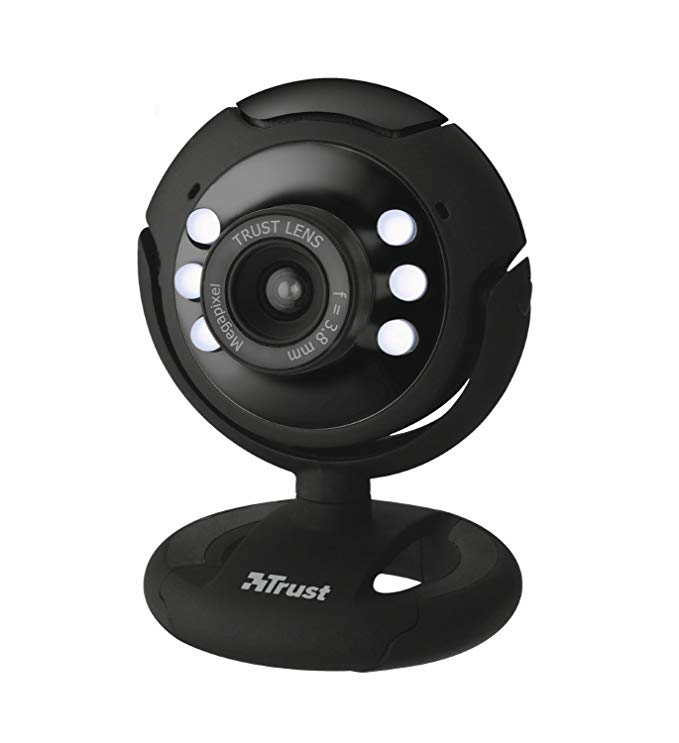
\includegraphics[width=0.25\textwidth]{Immagini/TrustCam.jpg}
	\caption{Camera utilizzata nello stato iniziale del progetto}
	\label{fig:TrustCam}
\end{figure}

È stato però notato che, utilizzando questa camera, non si era in grado di dare sufficienti garanzie di funzionamento stabile in alcune delle più comuni condizioni luminose e ambientali: infatti era alta la variabilità del comportamento della camera al variare delle condizioni luminose, il chè rendeva molto instabile il riconoscimento delle frecce.

Si è deciso quindi di passare ad una camera di tipo industriale, in grado di fornire delle prestazioni più stabili e affidabili.

La scelta è ricaduta sulla camera della casa produttrice \textit{IDS (Imaging Development System)}: si tratta del modello \textit{UI-1221LE-C-HQ} equipaggiata con la lente \textit{BM2420} prodotta dalla \textit{Lensagon} (\href{https://www.lensation.de/product/BM2420/}{lens datasheet}).
\begin{figure}[H]
	\centering
	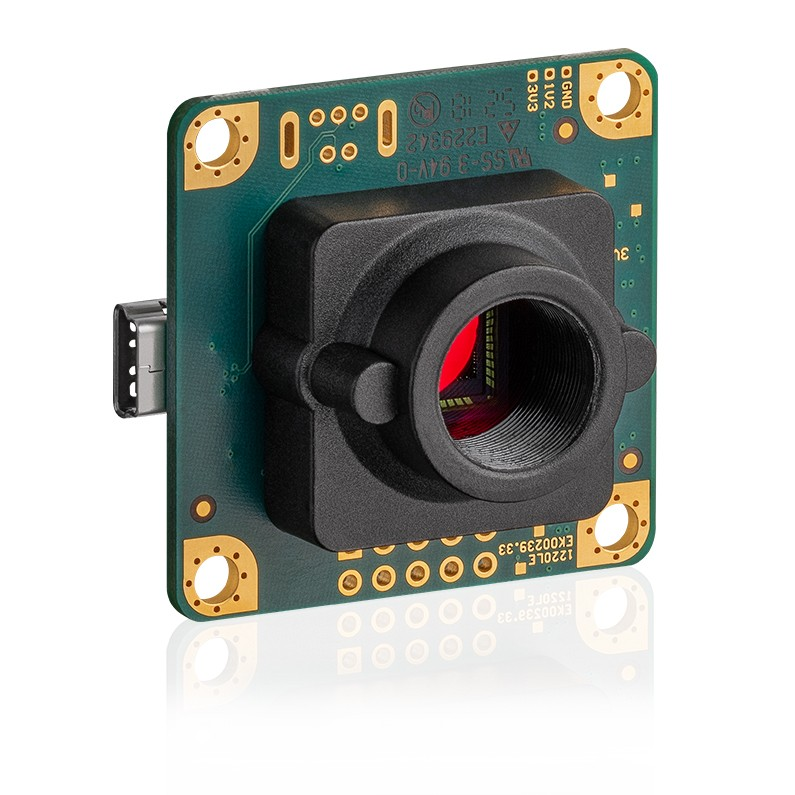
\includegraphics[width=0.3\textwidth]{Immagini/camera-usb2-ueye-le-rev2-boardlevel-m12-1.jpg}
	\caption{Camera utilizzata nello step successivo}
	\label{fig:UeyeCam}
\end{figure}

La camera in Fig.\ref{fig:UeyeCam} ha un'otturatore globale che permette di acquisire tutta l'immagine istantaneamente e non in modo progressivo come la camera  \textit{SpotLight Pro Webcam}.

\section{Come ottenere le immagini dalla camera?}
Per ottenere le immagini dalla camera è stato necessario iscriversi presso il sito web della casa produttrice e scaricare i driver necessari all'installazione e al funzionamento (\href{https://en.ids-imaging.com/manuals-ueye-software.html}{software}).

La videocamera ha diverse opzioni di acquisizione tra cui anche una grandezza dell'immagine diversa dal classico 640x480 pixel ma, per ragioni di semplicità, si è scelto di lasciare invariate le impostazioni di default.

In ogni caso è molto semplice verificare lo stato di funzionamento della camera stessa: è sufficiente, una volta scaricati e installati i software proprietari della casa produttrice, andare ad aprire il software \textit{uEyeDemo} e modificare le impostazioni in base alle proprie necessità.

E' necessario sottolineare come, per essere in grado di ottenere le immagini dalla camera, sia importante assicurarsi che \textit{l'ueye daemon} sia in funzione: esso parte automaticamente dal momento in cui si avvia il PC con la camera già connessa. Nel caso in cui essa venga connessa a caldo è necessario andare ad avviare il \textit{daemon} utilizzando questo comando da terminale, che mette in evidenza come si tratti di un comando per camera usb (nel caso si andasse a lavorare con camera ethernet, servirebbe andare a selezionare la giusta opzione, proposta a terminale):

\begin{quotation}
	\textsl{sudo /etc/init.d/ueyeusbdrc start}
\end{quotation}


\section{CPU consumption}
Un fattore importante nella scelta della camera è l'elevato tempo di utilizzo della CPU da parte della camera \textit{UI-1221LE-C-HQ}. In contrasto, la camera inizialmente scelta vantava un consumo di CPU nettamente inferiore e quindi che più si potrebbe adattare all'installazione su dispositivi mobili e con bassa potenza di calcolo.

\section{Posizionamento camera}

Durante i test e gli esperimenti svolti in laboratorio la videocamera è stata legata ad un palo metallico e fissata con un angolo di inclinazione rispetto ad esso di circa 35 gradi; l'altezza dal pavimento è, inoltre, di circa 83.5 cm

\section{Calibrazione}
La fase di calibrazione della camera permette di ricavare (alcuni o tutti) i parametri che permettono al modello \textit{pin-hole} di poter essere utilizzato per proiettare punti da coordinate mondo a coordinate camera. 

In inglese la calibrazione della camera, ovvero il ricavare i parametri intrinseci e/o estrinseci, si chiama \textit{Camera resectioning} in quando il concetto di Camera Calibration si può riferire anche al problema della calibrazione fotometrica del sistema.

Una telecamera è infatti generalmente modellata mediante il modello proiettivo centrale pinhole camera (o foro stenopeico). Tale modello è definito da due famiglie di parametri:

\begin{itemize}
	\item Parametri intrinseci (da tre a cinque): descrivono la telecamera indipendentemente dalla sua posizione nello spazio.
	\item Parametri estrinseci (sei): descrivono la posizione della telecamera nello spazio indipendentemente dalle sue caratteristiche interne.
\end{itemize}

Nel nostro caso specifico, per ottenere questi parametri di interesse, abbiamo sfruttato la forte interconnessione che la camera \textit{IDS} offre con l'ambiente ROS: infatti, installando uno specifico pacchetto software tramite il comando 

\begin{lstlisting}
	rosdep install camera_calibration
\end{lstlisting}

che permette di ottenere un insieme di pacchetti software scritti in \textit{Python}, i quali permettono di ottenere tutti i parametri di interesse.

Nello specifico, il comando da eseguire tramite il terminale è il seguente:

\begin{lstlisting}
	rosrun camera_calibration cameracalibrator.py --size 8x6 --square 0.108 image:=/camera/image_raw camera:=/camera
\end{lstlisting}

\begin{figure}[H]
	\centering
	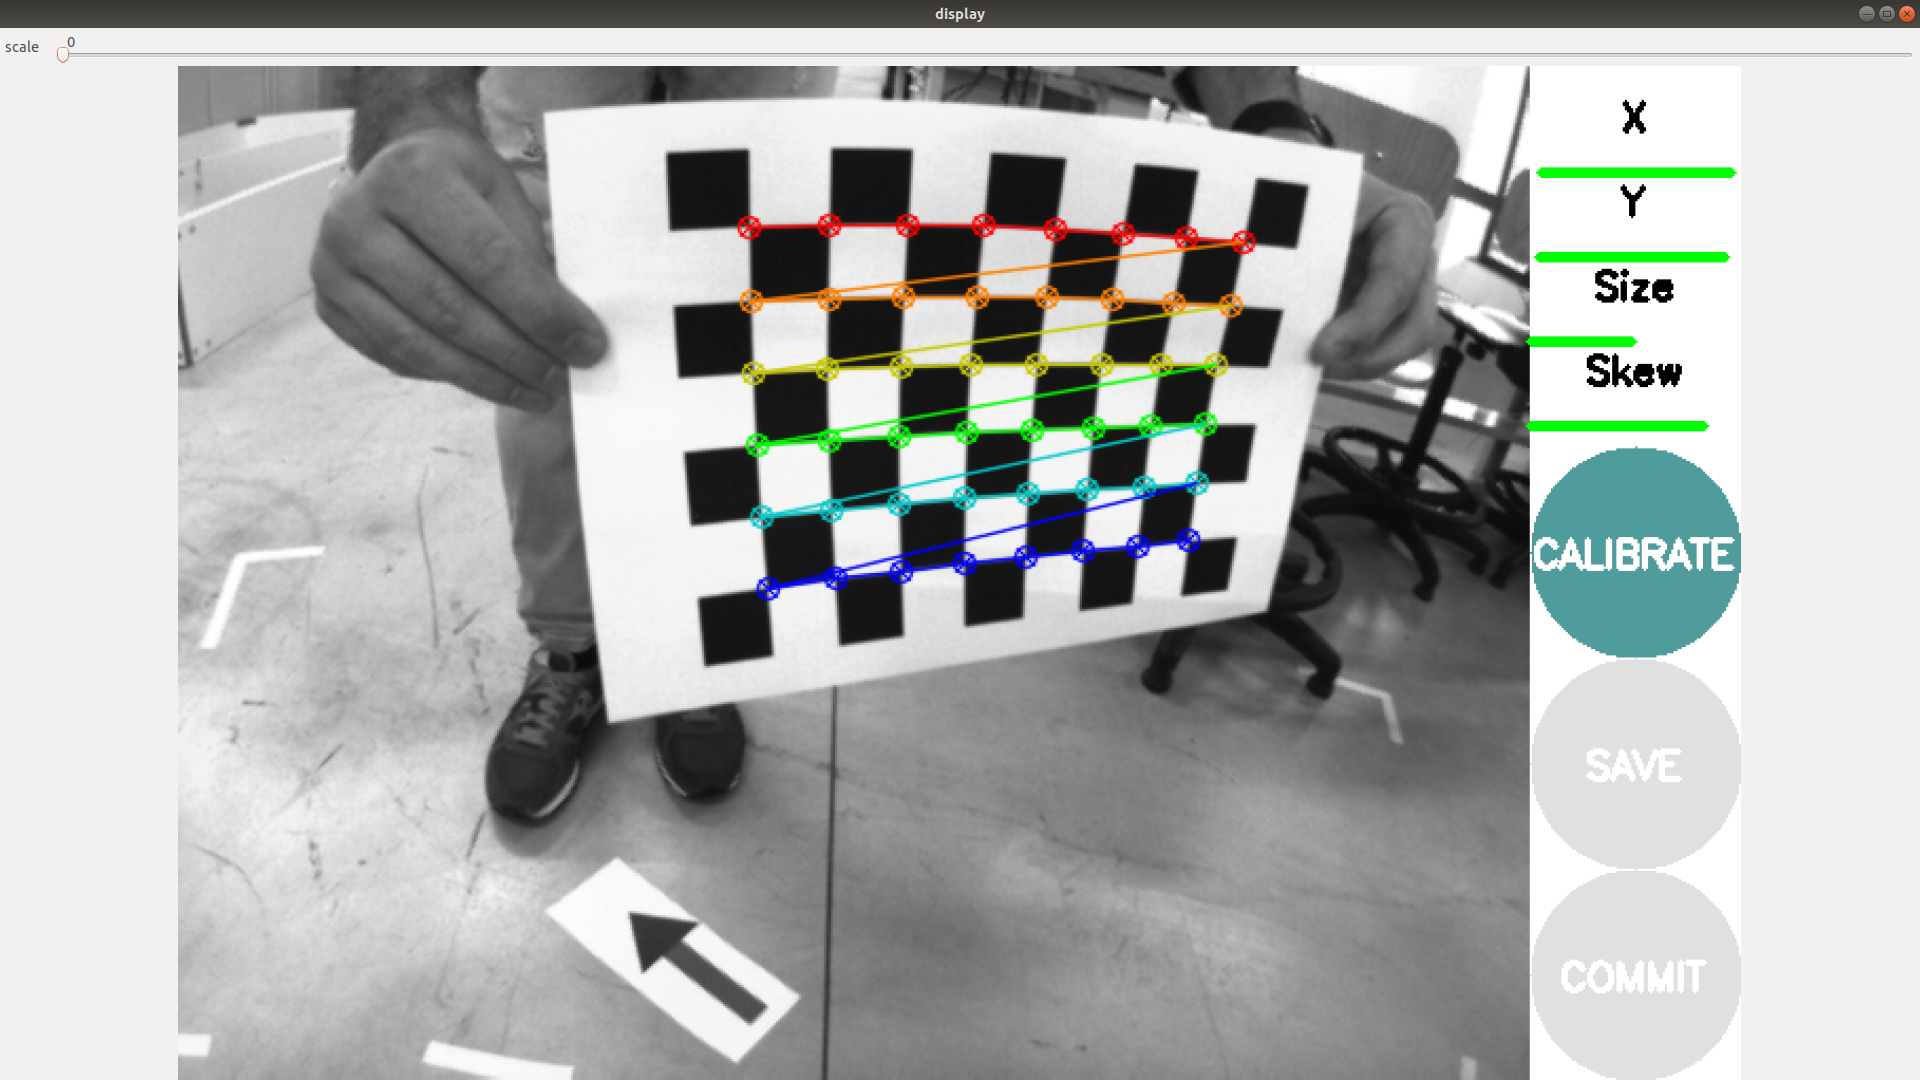
\includegraphics[width=0.8\textwidth]{Immagini/Calibration.png}
	\caption{Interfaccia grafica durante la calibrazione}
	\label{fig:calibrationInterface}
\end{figure}

Questi invece sono gli esiti forniti in uscita dal processo di calibrazione:

\begin{lstlisting}
	width
	640
	
	height
	480
	
	[narrow_stereo]
	
	camera matrix
	575.407063 0.000000 392.952424
	0.000000 572.733663 256.805741
	0.000000 0.000000 1.000000
	
	distortion
	-0.310832 0.140048 -0.005256 -0.007508 0.000000
	
	rectification
	1.000000 0.000000 0.000000
	0.000000 1.000000 0.000000
	0.000000 0.000000 1.000000
	
	projection
	517.612549 0.000000 400.977651 0.000000
	0.000000 540.829285 256.819184 0.000000
	0.000000 0.000000 1.000000 0.000000
\end{lstlisting}


